\begin{figure*}[t]
    \centering
    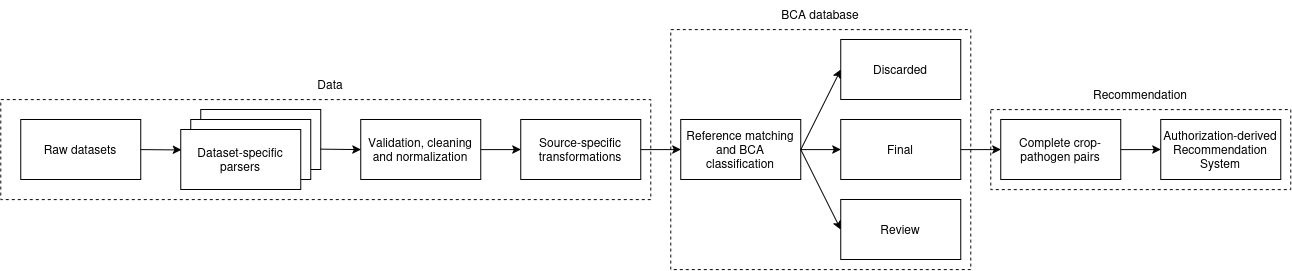
\includegraphics[width=\textwidth]{images/pipeline.png}
    \caption{Three-stage methodology: source parsing and normalisation, BCA database construction, and authorisation-derived BCA ranking.}
    \Description{A flow diagram showing raw datasets moving through dataset-specific parsers, validation and normalisation, source-specific transformations, reference matching and BCA classification, and final, review, or discarded outputs. Complete scientific crop--pathogen pairs from final records enter the authorisation-derived recommendation system.}
    \label{fig:pipeline}
\end{figure*}

\section{Methodology}\label{sec:methodology-or-approach}

The methodology has three stages:

\begin{enumerate}
    \item \textbf{Data}: collect, parse, and normalise authorisation records.
    \item \textbf{Commercial BCA database}: select BCA-related records and preserve their evidence and review state.
    \item \textbf{Recommendation}: rank microbial BCAs for a crop--pathogen query.
\end{enumerate}

Figure~\ref{fig:pipeline} shows how these phases connect: the Data phase produces the shared records, the Commercial BCA database phase assigns evidence states, and the Recommendation phase ranks BCA candidates for a query.

The stages are evaluated separately. This keeps data processing, database creation, and recommendation distinct.

As a preliminary screening step, the pipeline also applies a text classifier to the processed records. TF-IDF converts the
selected row fields into weighted sparse features, giving more weight to terms and phrases that distinguish a row and
less weight to terms repeated across the corpus. Logistic regression then learns a linear boundary between the
authorization-derived BCA-related and non-BCA classes. This classifier reproduces pipeline labels; its scores are not
biological efficacy estimates.
